\documentclass[12pt]{article}
\usepackage[utf8]{inputenc}
\usepackage[english]{babel}
\usepackage[T1]{fontenc}
\usepackage{amsmath}
\usepackage{amsfonts}
\usepackage{dsfont}
\usepackage{setspace}
\usepackage[dvipsnames]{xcolor}
\usepackage{graphicx}
\usepackage{mathtools}
\usepackage{float}
\usepackage{numprint}
\usepackage{url}
\usepackage{dirtree}
\usepackage{algorithmic}
\usepackage{algorithm}
\usepackage[hidelinks]{hyperref}
\hypersetup{
    linktoc=all,     %set to all if you want both sections and subsections linked
}

\usepackage[Glenn]{fncychap}
\usepackage{enumitem}
\usepackage{multicol}
\pagestyle{plain}
\usepackage{subfig}
\usepackage{siunitx}

% You can set the margine of the text by setting the top, bottom, left and right properties. Also, if using more than one columns, you can change the columnsep property to set the seperation space between two columns.
\usepackage[a4paper,top=30mm,bottom=30mm,columnsep=6mm,left=20mm,right=20mm]{geometry}

% uncommnet and change the following two commands to set seperation line width between coulmns.

% \setlength{\columnsep}{1cm}
% \setlength{\columnseprule}{0.6pt}

%########################## Paper Meta data#########################
% You can change the variables in the following section to set them globally thrghout the whole paper.

% Title of the paper
\newcommand{\papertitle}{Internship notes}
\newcommand{\shorttitle}{}

% Full name of the author(s)
\newcommand{\authorname}{Alexandre CHAUSSARD}

% Module code
\newcommand{\acmodulecode}{01/05/2023}

% Module name
\newcommand{\acmodulename}{}

% Name of the college
\newcommand{\accollegename}{Laboratoire de Probabilité, Statistiques et Modélisation}

% Date
\newcommand{\wrdate}{May 2023}
%########################## Paper Meta data#########################

\usepackage{fancyhdr}

\usepackage{biblatex}
\usepackage{algpseudocode}
\usepackage{textcomp}
\bibliographystyle{ieeetr}
\addbibresource{library.bib}

\pagestyle{fancy}
\fancyhead{}
\fancyhead[L]{\textsc{\shorttitle}}
\fancyfoot{}
\fancyfoot[R]{\thepage}
\fancyfoot[L]{\acmodulecode\  \textsc{\acmodulename}}
% \fancyfoot[C]{\thepage}
\renewcommand{\headrulewidth}{0.6pt}
\renewcommand{\footrulewidth}{0.6pt}


\title{\papertitle}
\author{\authorname}


\begin{document}
    
% general section    
\newcommand{\HRule}{\rule{\linewidth}{0.5mm}} 		
\begin{titlepage}
    \begin{center}
        %\vspace*{1cm}

        \center 
        \begin{figure}[H]
            \centering
            
\includegraphics[width=.5\textwidth]{images/logo_ipp.png}\label{fig:logo_ipp}
        \end{figure}
        
        % Document info
        \textsc{Laboratoire de Probabilité, Statistiques et Modélisation}\\[0.5cm]
        \textsc{\large May 2023}\\[2cm] 
        
        % Course Code
        \HRule \\[1cm]
        { \huge \bfseries Internship report notes}\\[1cm]			
        \HRule \\[.5cm]
        \large

        \vspace*{1cm}
        
        \emph{Master 2 - Data Science} \\[1cm]

        Alexandre CHAUSSARD  \\ [0.5cm]
        
    \end{center}
\end{titlepage}

\newpage
\tableofcontents
\newpage

\section{Introduction}


Given observations of random variables $(X,Y)$, we suppose that there exist another set of random variables $Z$ that we do not observe,
yet that characterize $(X,Y)$ conditionally to $Z$.
$Z$ is then called a latent variable, or a hidden variable. \\

For instance, if we observe the weights of a given population through $X$, and that we aim at inferring their height $Y$, knowing the
sex of each individual through $Z$ could improve our predictions on $Y$.
Hence, assuming that there exist a latent variable to a given model adds structure to the model while improving the explainability,
as $Z$ characterizes the behavior of our dataset.
Typically, clustering methods like KMeans or Gaussian Mixtures Models (GMM) provide a discrete $Z$ given the observations, which are
interesting in the sense that they provide a categorical representation of our data. \\

However, finding such $Z$ given the observations is not straight forward, and not all dataset respond to a latent process, and may be not even a discrete one. \\

During this research internship, we aim at exploring latent models with discrete latent space in order to analyze the microbiota structure.
Our first focus will be on various methods to conceive latent models like Expectation-Maximization and variational models.



\newpage

% EM
\section{Expectation-Maximization} \label{section:EM}

\subsection{Overview}

The Expectation-Maximization (EM) algorithm, first introduced in \cite{expectation_maximization_source}, is vast class of latent models.
It is based on the following smart decomposition of the data:
$$
\log p_{\theta}(X) = \underbrace{\mathbb{E}_{p_{\widehat{\theta}}(Z|X)}[\log p_{\theta}(X,Z)|X]}_{Q(\widehat{\theta}, \theta)} - \mathbb{E}_{p_{\widehat{\theta}}(Z|X)}[\log p_{\theta}(Z|X)|X]
$$

The idea behind this decomposition is that $\log p_{\theta}(X)$ is generally not tractable since it's an integral, while the complete likelihood $p_{\theta}(X,Z)$ is generally manageable.
Note that since $\log p_{\theta}(X)$ can not be computed, $\log p_{\theta}(Z|X)$ can't either by extension.
Hence, we introduce $\log p_{\widehat{\theta}}(Z|X)$ where $\widehat{\theta}$ is the maximum likelihood estimator of $\theta$:
$$
\widehat{\theta} = arg\max_{\theta} \log p_{\theta}(X)
$$

The main trick of the EM algorithm relies in the idea that $Q(\widehat{\theta}, \theta)$ is sufficient to compute a maximum likelihood estimator of $\theta$.
Indeed, consider the following algorithm:
\begin{algorithm}[H]
    \caption{Expectation-Maximization}
    \begin{algorithmic}
        \REQUIRE $\widehat{\theta}$
        \STATE Repeat until convergence
            \STATE \quad \textbf{Expectation}: compute $p_{\widehat{\theta}}(Z|X)$ to compute $Q(\widehat{\theta}, .)$
            \STATE \quad \textbf{Maximization}: $\widehat{\theta} = arg\max_{\theta} Q(\widehat{\theta}, \theta)$

        \RETURN{} $\widehat{\theta}$
    \end{algorithmic}

    \label{alg:em_algo}
\end{algorithm}

If we denote by $\widehat{\theta}^h$ the iterates of this algorithm, one can show using Jensen's inequality that:
$$
\log p_{\widehat{\theta}^{h+1}}(X) \geq \log p_{\widehat{\theta}^h}(X)
$$

As a result, the EM algorithm maximizes the likelihood, producing an estimator $\widehat{\theta}$ that is an MLE of $\theta$.
Note that we don't have a convergence certainty towards the best maximizer of the likelihood, only to a local maxima.
Hence, the EM algorithm is heavily sensitive to the initialization we pick. \\

All is required now is to choose a latent model so we can perform the EM algorithm, meaning that we have to define the distributions of the followings:
\begin{itemize}
    \item $Z \sim \mathcal{B}(K, \pi)$, conveniently set to a binomial of parameter $\pi$ so that it's discrete and simple to manage.
    \item $X|Z=k \sim p_{\gamma(k)}(X|Z=k)$, which is where we have the most choice to make.
\end{itemize}

In such models, $\theta = (\pi, \gamma(0), ..., \gamma(K))$.
In the next section, we will study a specific fork architecture of the gaussian mixture case.
\subsection{Gaussian Mixture Linear Classifier}

\subsubsection{Framework and computations}
Consider the case for which we observe $(X_i, Y_i)_{1 \leq i \leq n}$ i.i.d samples, where $X_i$ denotes a feature vector and $Y_i$ a label in a classification framework.
We aim at introducing a linear classifier that exploits a latent structure over $(X, Y)$, so that we have the following latent model:
\begin{itemize}
    \item $Z_i \sim \mathcal{B}(K, \pi)$, we note $\pi_k = \mathbb{P}(Z_i = k)$
    \item $X_i|Z_i=k \sim \mathcal{N}(\mu_k, \sigma_k I)$, we denote by $f_k(X_i)$ its density.
    \item $\mathbb{P}(Y_i = 1 | X_i, Z_i=k) = \sigma(W_{e,k}^T e_k + W_{x,k}^T X_i) = p_k(X_i)$, where $e_k$ denotes a vector from the canonical basis of $\mathbb{R}^K$.
\end{itemize}

As we want to perform the EM algorithm find an MLE of
$$
\theta = (\pi, \mu_1, ..., \mu_K, \sigma_1, ..., \sigma_K, W_{e,1}, ..., W_{e,K}, W_{x,1}, ..., W_{x,K})
$$
we start by computing the \textbf{expectation} step by assessing $p_{\widehat{\theta}}(Z_i = k|X_i,Y_i)$, using Bayes rules ($\hat{\pi}, \hat{p}, \hat{f}$ signify that we evaluate these quantities using the current estimate $\widehat{\theta}$):
$$
\begin{align}
    p_{\widehat{\theta}}(Z_i = k|X_i, Y_i) &= \frac{\hat{\pi}_k \hat{f}_k(X_i) \left(Y_i \hat{p}_k(X_i) + (1 - Y_i) (1 - \hat{p}_k(X_i)) \right)}{\sum_{j=1}^K \hat{\pi}_j \hat{f}_j(X_i) \left(Y_i \hat{p}_j(X_i) + (1 - Y_i) (1 - \hat{p}_j(X_i)) \right)}
    \\&= \tau_{ik}
\end{align}
$$

Now, we can safely evaluate $Q(\widehat{\theta}, \theta)$ for any $\theta$:
$$
\begin{align}
    Q(\widehat{\theta}, \theta) &= \mathbb{E}_{p_{\widehat{\theta}}(Z|X)}[\log p_{\theta}(X, Y, Z) | X] \\
    &= \sum_{i=1}^n \sum_{k=0}^K \log p_{\theta}(X_i, Y_i, Z_i = k) \tau_{ik} \\
    &= \sum_{i=1}^n \sum_{k=0}^K (\log \pi_k + \log f_k(X_i) + Y_i \log p_k(X_i) + (1 - Y_i) \log (1-p_k(X_i))) \tau_{ik} \\
\end{align}
$$

The \textbf{maximization} step now consists in deriving $Q(\widehat{\theta}, \theta)$ regarding each parameters in $\theta$
so that we obtain an either explicit value or iterative procedure to compute the next iterate of $\widehat{\theta}$.
\begin{itemize}
    \item Maximization regarding $\pi_k$ under constraint that $\sum_{k=0}^K \pi_k = 1$ can be solved explicitly using Lagrange duality:
    $$
    \pi_k^* = \frac{1}{n} \sum_{i=1}^n \tau_{ik}
    $$
    \item Maximization regarding $(\mu_k, sigma_k)$ is given by the maximum of likelihood estimator on $\sum_{i=1}^n \tau_{ik} \log f_{k}(X_i)$:
    $$
    \begin{align}
        \mu_k^* &= \frac{1}{\sum_{i=1}^n \tau_{ik}} \sum_{i=1}^n \tau_{ik} X_i \\
        \sigma_k^* &= \frac{1}{\sum_{i=1}^n \tau_{ik}} \sum_{i=1}^n \tau_{ik} (X_i - \mu_k^*)(X_i - \mu_k^*)^\top
    \end{align}
    $$
    \item Maximization regarding $(W_{e,k}, W_{x,k})$ is not explicit, and requires a fixed point algorithm like gradient descent to determine an estimate of the optimal parameters.
    The iterations using full batch gradient descent are given below, with learning rate $\alpha$:
    $$
    \begin{align}
        W_{e,k}^{l+1} &\leftarrow W_{e,k}^{l} - \alpha \sum_{i=1}^n (p_k(X_i) - Y_i) \tau_{ik} e_k \\
        W_{x,k}^{l+1} &\leftarrow  W_{x,k}^{l} - \alpha \sum_{i=1}^n (p_k(X_i) - Y_i) \tau_{ik} X_i
    \end{align}
    $$
    Each iteration should be confronted to the maximization criterion, so that each iterate improves $Q(\widehat{\theta}, \theta)$:
    $$
    Q(\widehat{\theta}^{l+1}, \theta) \geq Q(\widehat{\theta}^{l}, \theta)
    $$
    In the end, only the best improvement iterate is kept for $W_{e,k}^*$ and $W_{x,k}^*$. Note that other methods could be used like SGD or CMAES as implemented during the internship.
\end{itemize}

After the maximization, we can update $\widehat{\theta}$ with the previously computed parameters, and redo the (E) and (M) steps up to convergence.
The convergence can be measured relatively to $ Q(\widehat{\theta}, \theta)$, so that for a threshold $\epsilon$, we can use the following stopping criterion:
$$
\frac{|Q(\widehat{\theta}^{h+1}, \widehat{\theta}^{h}) - Q(\widehat{\theta}^{h}, \widehat{\theta}^{h})|}{|Q(\widehat{\theta}^{h}, \widehat{\theta}^{h})|} \leq \epsilon
$$

We now have a ready-to-go Gaussian Mixture Linear Classifier that we can benchmark on an suited dataset against other common methods.

\subsubsection{Dataset generation}

Before we benchmark the Gaussian Mixture Linear Classifier, we need to generate a dataset that is well suited to its usage.
Hence, we set random parameters for $\theta$ and generate a new dataset following the latent framework we have set previously:
\begin{itemize}
    \item For all $k \leq K$, generate $n/K$ points following a gaussian parameterized by $(\mu_k, \sigma_k I)$.
    $X$ is given by each point coordinate, $Z$ by the gaussian from which the point was generated.
    \item For each sample, characterized by ($X_i$, $Z_i$), draw the label of the sample as $Y_i \sim \mathcal{B}(\sigma(W_{e,Z_i}^T e_{Z_i} + W_{x,Z_i} ^ T X_i))$.
\end{itemize}

The following figure illustrates a generation with $K=2$:
\begin{figure}[H]
    \center
    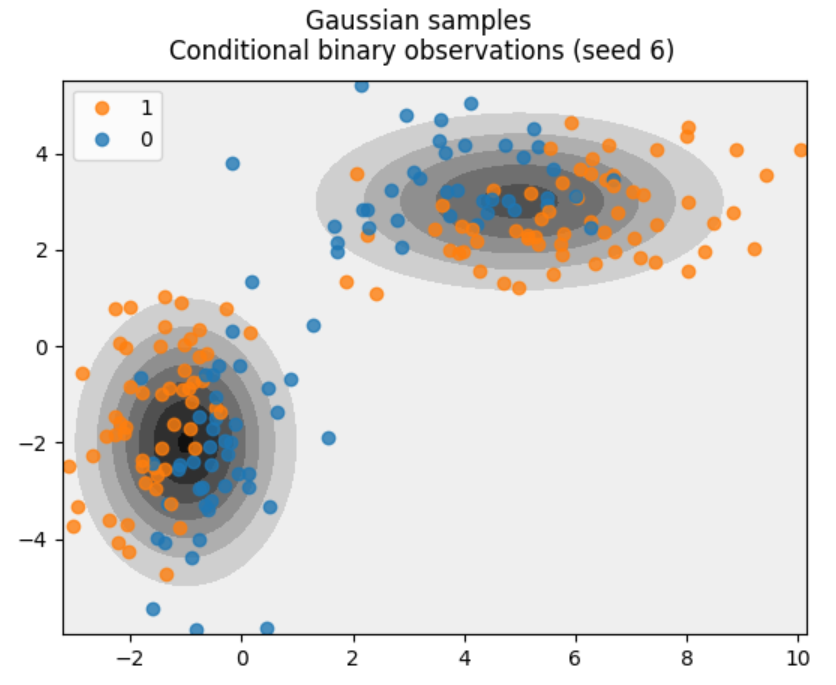
\includegraphics[scale=0.7]{images/samples_gmm_lc}
    \caption{Generated samples out of $K=2$ gaussians, labelized using a logistic model (label 1 or 0).
    The density of the hidden gaussians is represented in the background using shades of grey (black intense, white almost 0)}
    \label{fig:samples_gmm_lc}
\end{figure}

Note on the previous figure \ref{fig:samples_gmm_lc} that the limit between the labels in each subset gaussian is not sharp,
as it is sorted out of a probabilistic modelisation (logistic).
Consequently, an interesting observation can be made as we force the gaussians to have small values of mean and variance.
Indeed, as shown on the next figure, if we take the same parameters as previously and divide them by a factor 10,
the logistic model is ill conditioned.
\begin{figure}[H]
    \center
    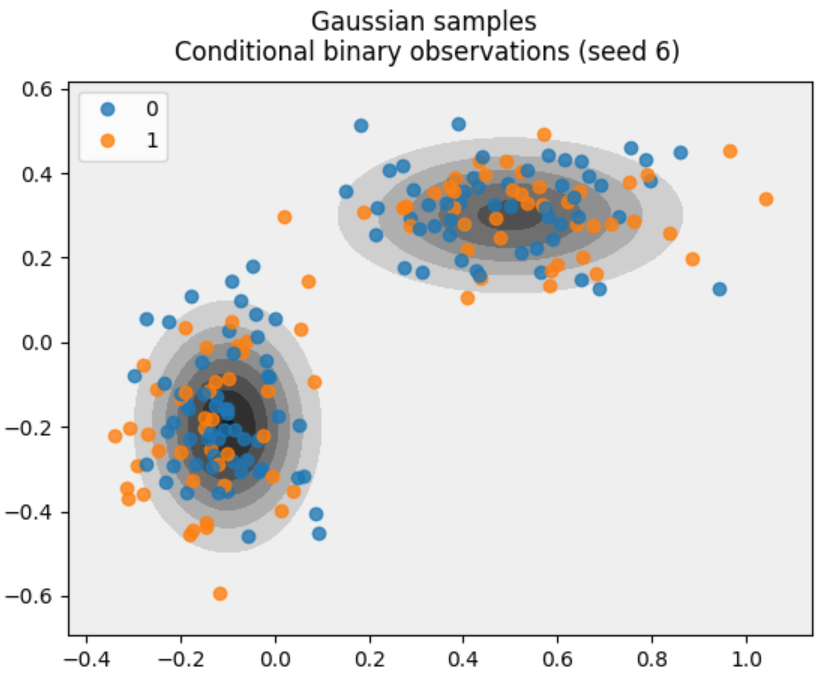
\includegraphics[scale=0.7]{images/samples_gmm_lc_badconditioning}
    \caption{Generated samples out of $K=2$ gaussians, using the same parameters as for figure \ref{fig:samples_gmm_lc} divided by a factor 10.}
    \label{fig:gmm_lc_badconditioning}
\end{figure}

All points are close to the frontier in terms of norm on figure \ref{fig:gmm_lc_badconditioning}.
Since we do not exploit any normalization term in the sigmoid modelization, this leads to a blurry area in which the linear separation model is not useful at all.
This situation is heavily problematic as it prevents us from performing a general benchmark on that dataset.
Indeed, the further larger the variance is, with sufficient samples, the better the linear approximation will be and therefore the better the modelization gets.
On the contrary, with smaller variance the linear model isn't descriptive of the generated samples as they are all close to the frontier, therefore with heavily noisy labelization.
\subsection{Dirichlet Mixture Linear Classifier}

\subsubsection{Framework and objectives}

In the previous section, we have derived a very classical model (Gaussian Mixture Model) into a linear classifier using the EM algorithm.
However, gaussian latent modelization is far from general, and may not be suited to our specific usage on the microbiota.
Indeed, after performing the previous method onto our microbiota dataset, it turned out to be performing just as bad as the classical logistic regression, no matter the chosen latent space dimension.
Therefore, we deduce that the gaussian latent modelization is not adapted to our practical settings. \\

As we analyze the data, we observe that each $X_i$ belongs to the simplex.
A natural distribution supported on the simplex is the Dirichlet distribution, parameterized by $\alpha = (\alpha_1, \dots, \alpha_p)$ where $p$ is the dimension of $X_i$.
We denote the dirichlet distribution by $\mathcal{D}(\alpha)$, for which the density is given by the following:
$$
f(x|\alpha) = \frac{\Gamma \left( \sum_{j=1}^p \alpha_j \right)}{\Pi_{j=1}^p \Gamma (\alpha_j)} \Pi_{j=1}^p x_j^{\alpha_j - 1}
$$
where $\Gamma$ denotes the gamma function.
For notation simplicity, we also introduce the digamma function that will play a key role in our model:
$$
\psi(\alpha) = \frac{d}{d \alpha} \log \Gamma(\alpha) = \frac{\Gamma '(\alpha)}{\Gamma(\alpha)}
$$

Since we are doing a Dirichlet mixture model, we have $K$ Dirichlet distributions to handle.
We introduce the notation $\alpha^{(k)}$ to parameterize the $k$-th Dirichlet distribution. \\

As previously, we first perform the \textbf{expectation} step obtain the same result with a different conditional a priori distribution on $X|Z$:
$$
\begin{align}
    p_{\widehat{\theta}}(Z_i = k | X_i, Y_i) &= \frac{\hat{\pi}_k f(X_i | \hat{\alpha}^{(k)}) (Y_i \hat{p}_k(X_i) + (1 - Y_i)(1 - \hat{p}_k(X_i)))}{\sum_{j=1}^K \hat{\pi}_j f(X_i | \hat{\alpha}^{(j)}) (Y_i \hat{p}_j(X_i) + (1 - Y_i)(1 - \hat{p}_j(X_i)))} \\
                                             &= \tau_{ik}
\end{align}
$$

We can now evaluate $Q(\widehat{\theta}, \theta)$ for any $\theta$, which enables us to perform the \textbf{maximization} step:
\begin{itemize}
    \item The maximization over $pi_k$ under the simplex constraint $\sum_{k=1}^k \pi_k = 1$ is again given by Lagrange duality as:
        $$
        \pi_k^* = \frac{1}{n} \sum_{i=1}^n \tau_{ik}
        $$
    \item The maximization over $\alpha^{(k)_j}$ is not straightforward on the other hand, and requires a fixed point algorithm.
          Indeed, deriving over $\alpha^{(k)_j}$ we obtain:
        $$
        \begin{align}
            \partial_{\alpha^{(k)}_j} Q(\widehat{\theta}, \theta) &= \sum_{i=1}^n \left(\psi \left(\sum_{l=0}^K \alpha_{l}^{(k)} \right) - \psi(\alpha_{j}^{(k)}) + \log x_{ij} \right) \tau_{ik} \\
                                                                  &= \left(\psi \left(\sum_{l=0}^K \alpha_{l}^{(k)} \right) - \psi(\alpha_{j}^{(k)})\right) \sum_{i=1}^n \tau_{ik} + \sum_{i=1}^n \tau_{ik} \log x_{ij}
        \end{align}
        $$
        Hence, as we look for $\partial_{\alpha^{(k)}_j} Q(\widehat{\theta}, \theta) = 0$, we obtain:
        $$
        \psi(\alpha_{j}^{(k)}) - \psi \left(\sum_{l=0}^K \alpha_{l}^{(k)} \right) = \frac{\sum_{i=1}^n \tau_{ik} \log x_{ij}}{\sum_{i=1}^n \tau_{ik}}
        $$
        Thankfully, \cite{dirichlet_digamma_trick} provides a few tricks to solve iteratively such equation, so that we can iterate as follows (5 steps are sufficient to obtain high-accuracy solution according to \cite{dirichlet_digamma_trick}):
        $$
        \begin{align}
            \alpha_{j}^{(k)} &\leftarrow \psi^{-1}\left(\frac{\sum_{i=1}^n \tau_{ik} \log x_{ij}}{\sum_{i=1}^n \tau_{ik}} + \psi \left(\sum_{l=0}^K \hat{\alpha}_l^{(k)} \right)  \right) \\
            \hat{\alpha}_j^{(k)} &\leftarrow \alpha_{j}^{(k)}
        \end{align}
        $$
        However, this solution is a lower bound to the true objective, which makes our EM a generalized version of it.
    \item The maximization over $(W_{e,k}, W_{x,k})$ is also given by a fixed point algorithm, which ends up being the same computation as previously for the Gaussian case:
        $$
        \begin{align}
            W_{e,k}^{l+1} &\leftarrow W_{e,k}^{l} - \alpha \sum_{i=1}^n (p_k(X_i) - Y_i) \tau_{ik} e_k \\
            W_{x,k}^{l+1} &\leftarrow  W_{x,k}^{l} - \alpha \sum_{i=1}^n (p_k(X_i) - Y_i) \tau_{ik} X_i
        \end{align}
        $$
\end{itemize}

\subsubsection{Dataset generation}

Now that we have defined the EM algorithm in the previous section, we aim at generating a dataset to benchmark the dirichlet mixture classifier.
Following a similar procedure as for the gaussian case, we are able to generate a dataset that matches a dirichlet mixture and is labeled following the sigmoid modelisation.
The next figure illustrates a given generation:
\begin{figure}[H]
    \center
    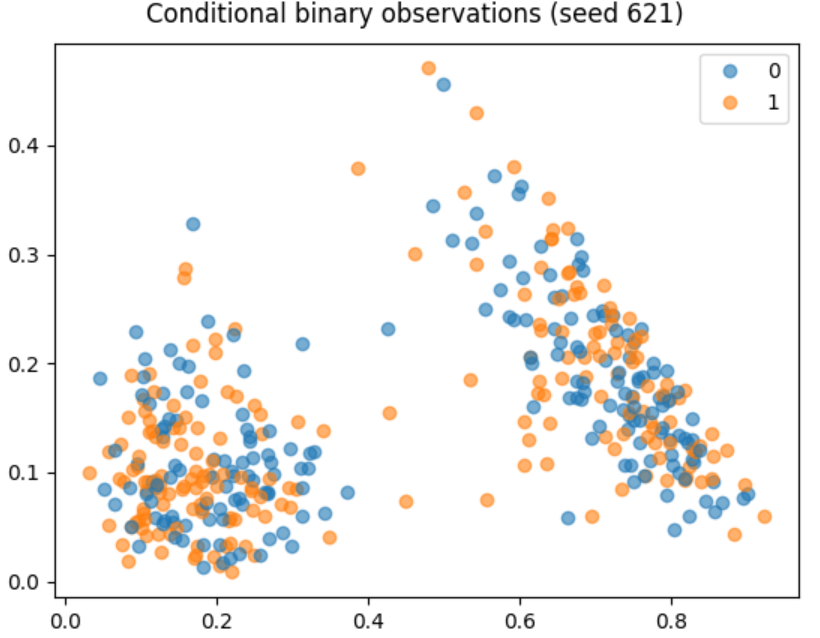
\includegraphics[scale=0.7]{images/samples_dirichlet_lc}
    \caption{Generated samples out of $K=2$ dirichlet distributions, labelized using the sigmoid modelisation on $\mathbb{P}(Y_i = 1)$.}
    \label{fig:dirichlet_lc_badconditioning}
\end{figure}

As previously, since the data lives in the simplex, they are too close to the border of the next label set, which ends up creating a blurry dataset for which the
linear model is not relevant anymore.

% Discrete VAE
\newpage
\section{Variational methods}

In this section, we aim at resourcing some variational methods that we are going to use in this study.
\section{Variational Auto-Encoders}

\subsection{Framework and optimization objective}

We are interested in another kind of latent models, this time based on variational inference
results to achieve a new kind of deep latent structure: the Variational Auto-Encoder (VAE).
These latent models were introduced in 2013 by Kingma, better described in a more in depth paper in 2019: \cite{kingma2019introduction}

Once again, we assume the observations $X$ to be modelizable by a given distribution
parameterized by $\theta$:

$$
X \sim p_{\theta}(x)
$$

Determining $\theta$ holds to find one $\theta^*$ that would optimize a given objective, generally chosen as the maximum of likelihood. Indeed, if $\theta^* \in arg\max_{\theta} p_{\theta}(x)$, then such $\theta^*$ maximizes the density around the dense areas of the observations, which makes them highly likely to happen under such distribution $p_{\theta^*}$. Hence, the maximum likelihood is a natural criterion:
$$
\theta^* \in arg\max_{\theta} p_{\theta}(x)
$$

However, such modelization does not include a latent structure. As a result, we try to enforce it by rewriting the objective as follows:

$$
p_{\theta}(x) = \int_{\mathcal{Z}} p(x,z) dz 
$$

Using Bayes decomposition, we obtain a computable objective:
$$
p_{\theta}(x,z) = p_{\theta}(z) p_{\theta}(x|z)
$$

Recall that the prior $p_{\theta}(z)$ and the a priori $p_{\theta}(x|z)$ are defined by the framework (ex: Bernoulli prior and Gaussian posterior gives the Gaussian mixture framework). However, the computation of the evidence $p_{\theta}(x)$ is generally intractable in practice, which also leads to a non-tractable posterior distribution: $p_{\theta}(z|x)$. As a result, not being able to compute the evidence leads to not being able to provide a gradient regarding $\theta$, so we can not perform the backpropagation in a deep learning approach.

Note that there exist approximate inference techniques to compute the evidence and the posterior, but these are quite expensive and often yield poor convergence results.

To overcome this issue, we introduce a smart rewriting of the objective using variational inference. Indeed, let $q_{\Phi}(z|x) \approx p_{\theta}(z|x)$ to be learnt over $\Phi$, one can write:
$$
\begin{align}
    \log p_{\theta}(x) &= \mathbb{E}_{q_{\Phi}(z|x)}[\log p_{\theta}(x)] \\
    &= \mathbb{E}_{q_{\Phi}(z|x)}\left[\log \frac{p_{\theta}(x)}{q_{\Phi}(z|x)} \frac{q_{\Phi}(z|x)}{p_{\theta}(z|x)}\right]
    \\
    &= \underbrace{\mathbb{E}_{q_{\Phi}(z|x)} \left[\log \frac{p_{\theta}(x)}{q_{\Phi}(z|x)}\right]}_{ELBO(q_\phi(z|x), p_{\theta}(x,z))} + D_{KL}\left[q_{\Phi}(z|x) \Vert p_{\theta}(z|x)\right]
\end{align}
$$

The first term of that decomposition is generally called the Evidence Lower BOund (ELBO), as it marks a lower bound to the evidence $\log p_{\theta}(x)$ since the KL divergence is a positive quantity:
$$
\log p_{\theta}(x) \ge ELBO(q_\phi(z|x), p_{\theta}(x,z))
$$

$q_{\Phi}(z|x)$ is an approximation of the true posterior $p_{\theta}(z|x)$ that we aim at learning in a family of distributions. For instance, 
$$
q_{\Phi}(.|x) \sim \mathcal{N}(\mu(x), \Sigma(x))
$$ 
would be an approximation of the true posterior by a Gaussian distribution. Notice that the true posterior may very not likely be Gaussian, which creates a first complexity error in our model.

Despite being a lower bound on the true maximum likelihood objective, the ELBO is actually tractable. Indeed, as we continue the computation:
$$
\begin{align}
    ELBO(q_\phi(z|x), p_{\theta}(x,z)) &= \mathbb{E}_{q_{\Phi}(z|x)}[\log p_{\theta}(x,z)] - \mathbb{E}_{q_{\Phi}(z|x)}[\log q_{\Phi}(z|x)] \\
    &= 
\mathbb{E}_{q_{\Phi}(z|x)}[\log p_{\theta}(x|z)] - D_{KL}[\log q_{\Phi}(z|x) \Vert p_{\theta}(z)] \\\end{align}
$$

Another remarkable fact, is that when maximizing the ELBO, we are actually minimizing the KL divergence between the estimated and the true posterior. Hence, one can define the ELBO as a suboptimal objective to our problem that we get to maximize to obtain $(\Phi^*, \theta^*)$, the parameters of our model.

\subsection{Reparameterization trick}

Even though the gradient of the ELBO is well defined for $\theta$, it is not possible to compute it relatively to $\Phi$ it requires samples from the approximation to the posterior $q_{\Phi}(z|x)$ to compute $\mathbb{E}_{q_{\Phi}(z|x)}[\log p_{\theta}(x|z)]$. 

Since, sampling is not a differentiable operation, we make use of the change of variable formula, so that for a bijective transformation $z = \phi_x(\epsilon)$, we get:
$$
p(z) = p(\epsilon) \det \left| \frac{\partial \epsilon}{\partial z}\right|
$$

Hence, if we take $\epsilon$ a random variable of density $p(\epsilon)$ that does not depend on $\theta$, $\Phi$ nor $x$, so that $z = \phi_x(\epsilon)$, for any $L_1$ function $f$,
$$
\mathbb{E}_{q_{\Phi}(z|x)}[f(z)] = \mathbb{E}_{p(\epsilon)}[f(z)]
$$

As a result, the samples are not obtained through $q_{\Phi}$ anymore but through $p(\epsilon)$, so that can safely perform derivation of the ELBO relatively to $\Phi$ and backpropagate our gradient through the network.

\subsection{Architecture}

The vanilla architecture of the VAE is described by the following illustration:

[ILLUSTRATION VAE]

The first part is generally called the encoder, as it turns a sample $x$ into its latent representation $z$ by modelizing the posterior $q_{\Phi}(z|x)$. The second part is then called the decoder, as it throws a latent representation in the sample space. The latest can even serve as a generative architecture, as one can sample from the latent space through $q_{\Phi}(z|x)$, and decode it to obtain a new sample.

As we can see more clearly in that illustration, we can see that $\Phi$ and $\theta$ are trained jointly through the ELBO, both serving for one part of the VAE at a time.

The training procedure is straightforward: the entry is a sample $x$ and the output objective is the same sample $x$. We aim at train the VAE for learning the data space and its latent representation by learning how to reconstruct the samples through it.




\newpage
\section{VQ-VAE}

\subsection{Quick overview}

Introduced in \cite{vq_vae_paper}, VQ-VAE architecture provides a framework to compute
discrete posterior distributions $q_{\Phi}(z|x)$.
To compare that model with the VAE, we start by introducing the architecture of the model for which an illustration is given below:

\begin{figure}[H]
    \centering
    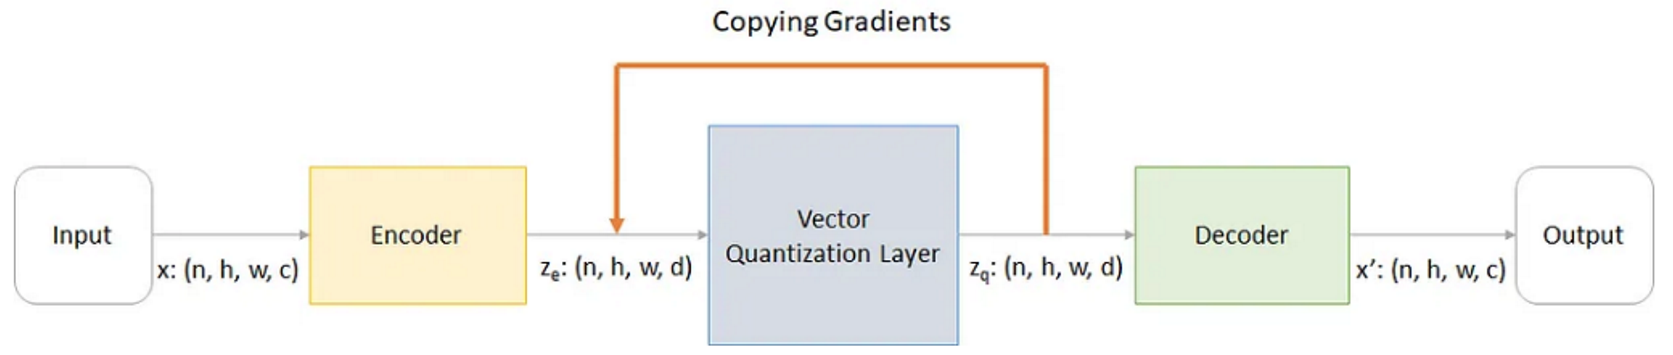
\includegraphics[width=.9\textwidth]{images/vq_vae_architecture}
    \caption{VQ-VAE architecture (source: Medium)}
    \label{fig:vq_vae_architecture}
\end{figure}

As we can see on figure \ref{fig:vq_vae_architecture}, the major difference with the vanilla VAE architecture
lies in the vector quantization step which enables to project the output of the encoder denoted by $z_e(x)$
onto a discrete embedding dictionary $(e_1, \dots, e_K)$ by a simple distance argument:
$$
k = arg\min_{j} \Vert z_q(x) - e_j \Vert_2, \quad z_q(x) = e_k
$$

The projection of $z_e(x)$ on that discrete dictionary is denoted by $z_q(x)$, and serves as the input of the decoder.
For further visual representation of the vector quantization layer, an illustration is given below.

\begin{figure}[H]
    \centering
    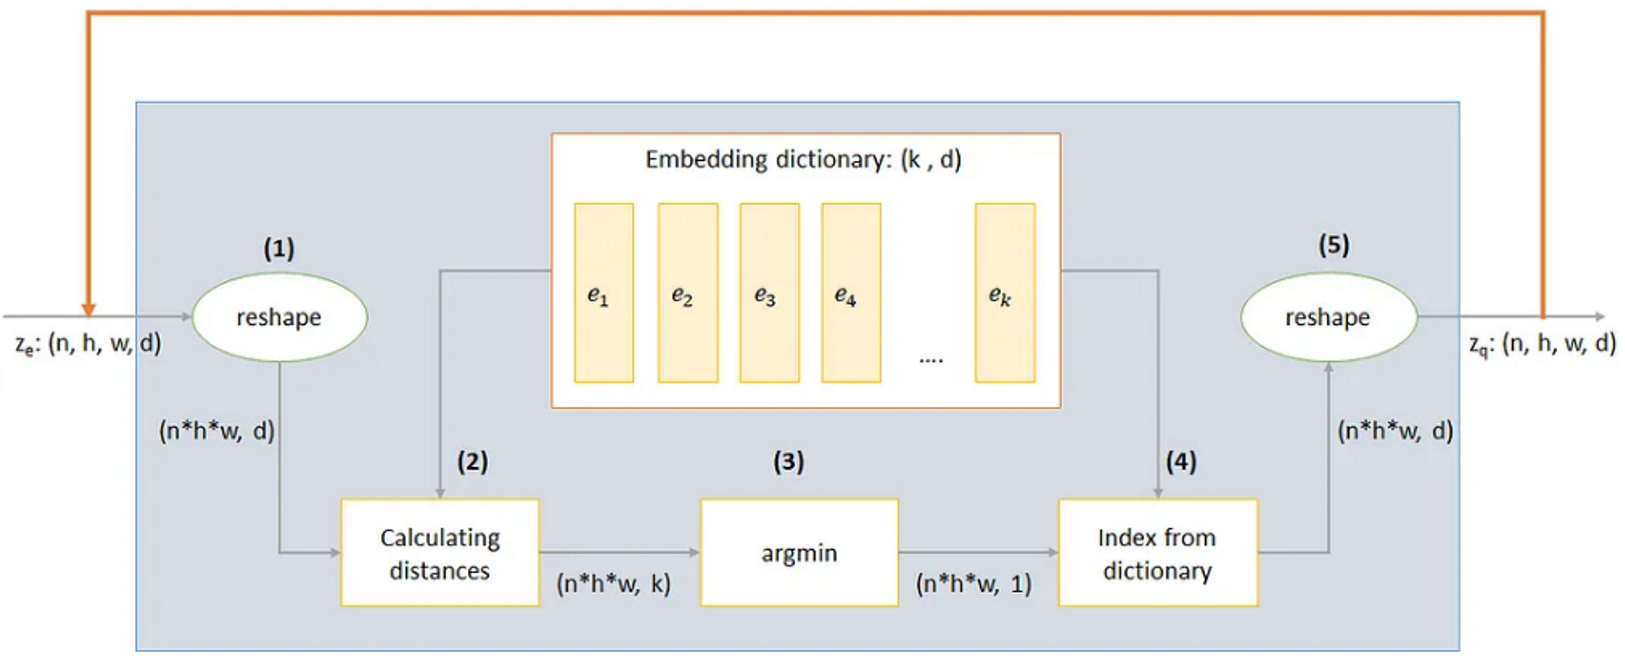
\includegraphics[width=.7\textwidth]{images/vq_vae_quantization}
    \caption{Architecture of the VQ-VAE: quantization layer (source: Medium)}
    \label{fig:vq_vae_quantization}
\end{figure}

Looking at the previous figures, we can grasp the challenge of backpropagation in such model with discrete prior and posterior.
In the next section, we enter in the mathematical definition of the objective and how to train this architecture.

\subsection{Framework and optimization objective}

Contrary to the vanilla VAE, we have the following categorical distributions assumption:
\begin{itemize}
    \item The prior $p_{\theta}(z)$ is categorical.
          In the original paper, it is taken as uniform supported in $\{1, \dots, K\}$ during the training.
          When the training is over, it is fit to an autoregressive distribution through a PixelCNN (see \cite{pixel_cnn_paper}).
          It is left as an exploration research field to be able to learn the prior while training the model.
    \item The posterior $q_{\Phi}(z|x)$ is categorical and set to the following:
          $$
          q_{\Phi}(k|x) = \mathds{1}_{\{k = arg\min_{j} \Vert z_q(x) - e_j \Vert_2\}}
          $$
\end{itemize}

This modelization of the posterior enables to obtain a discrete latent space, but it does not allow to differentiate regarding $\Phi$.
As a result, the authors suggest two possible strategies:
\begin{itemize}
    \item \textit{Straight-through}: propagate the gradient through the discrete part (vector quantization layer) without changing it.
          The intuition is that the gradient propagated from the encoder contains sufficient information to update the encoder accordingly, but this is just intuition.
    \item \textit{Subgradient}: compute the subgradient of the quantization layer (unexplored yet)
\end{itemize}

The optimization objective of the VQ-VAE is based on the ELBO, that one can compute as follow:
$$
\begin{align}
    ELBO(q_{\Phi}(z|x), p_{\theta}(z|x)) &= \mathbb{E}_{q_{\Phi}(z|x)}[\log p_{\theta}(x,z)] - \mathbb{E}_{q_{\Phi}(z|x)}[\log q_{\Phi}(z|x)] \\
    &= \mathbb{E}_{q_{\Phi}(z|x)}[\log p_{\theta}(x|z)] - D_{KL}[q_{\Phi}(z|X) \Vert p_{\theta}(z)]
\end{align}
$$

Notice then that:
\begin{itemize}
    \item Since $q_{\Phi}(k|x) = \mathds{1}_{\{k = arg\min_{j} \Vert z_q(x) - e_j \Vert_2\}}$, we have:
          $$
          \begin{align}
              \mathbb{E}_{q_{\Phi}(z|x)}[\log p_{\theta}(x|z)] = \log p_{\theta}(x|z_q(x))
          \end{align}
          $$
    \item Since $Z \sim \mathbb{U}(\{1, ..., K\})$, $\mathbb{P}(Z=k) = \frac{1}{K}$.
          Also, notice that $q_{\Phi}(z_q(x)|x) = 1$ by definition of $q_{\Phi}(z|x)$ and $z_q(x)$.
          Combining those results, we obtain:
          $$
          \begin{align}
              D_{KL}[q_{\Phi}(z|x) \Vert p_{\theta}(z)] &= \mathbb{E}_{q_{\Phi}(z|x)}\left[\log \frac{q_{\Phi}(z|x)}{p_{\theta}(z)} \right] \\
              &= \log \frac{q_{\Phi}(z_q(x)|x)}{p_{\theta}(z_q(x))} \\
              &= \log K
          \end{align}
          $$
          Therefore, this KL divergence does not impact the optimization objective as it does not depend on ($\theta$, $\Phi$).
\end{itemize}

Computing the previous quantities, we would obtain the following suboptimal objective for the VQ-VAE:
$$
ELBO(\Phi, \theta) = log p_{\theta}(x|z_q(x))
$$

However, such objective does not enable to learn the dictionary since we use a straight-through approach over the quantization layer.
To update the dictionary, the authors suggest to add the following term to the loss:
$$
\Vert sg[z_e(x)] - e \Vert_2^2
$$
Where $sg$ denotes the stop-gradient operator, meaning we do not consider any gradient after the given operation.
\medskip

Finally, to prevent embedding space over expansion, the authors suggest the addition of a commitment loss parameterized by $\beta > 0$:
$$
\beta \Vert z_e(x) - sg[e] \Vert_2^2
$$
Indeed, the embedding space was unconstrained so far, so its dimension could grow arbitrarily.
Intuitively, adding that term forces the model to commit to a given embedding.
\medskip

Overall, we obtain this final objective to maximize:
$$
\mathcal{L}(\theta, \Phi) = \log p_{\theta}(x|z_q(x)) + \Vert sg[z_e(x)] - e \Vert_2^2 + \beta \Vert z_e(x) - sg[e] \Vert_2^2
$$

\subsection{Discussion over some limiting aspects}

Even though the previous objective seems natural, we only rigorously justified the first term thanks to the ELBO.
Indeed, the dictionary update loss as well as the commitment loss keep dropping out from nowhere, while they seem necessary to ensure the training of our model.
\medskip

Furthermore, we did not really deal with the non differentiability of the vector quantization loss, and the straight-through estimator
can definitely be criticized about what information it actually provides to the encoder to update appropriately.
\medskip

Finally, the usage of the PixelCNN after the training seems very unnatural, and could significantly boost the model as the PixelCNN did show amazing performances so far.
\newpage
\section{PixelCNN}

\subsection{Overview}

Introducing the VQ-VAE, we have seen that an under-table tool that was being used is the Pixel CNN,
first introduced in \cite{pixel_cnn_paper}.
In the context of the VQ-VAE, it plays a major role after training by learning the prior $p(z)$, that was set
to a discrete uniform previously.
This makes a drastic difference with the VAE, as we are not setting the prior ourselves as it's being learnt and modeled by the PixelCNN in this process.
\medskip

Indeed, the PixelRNN/PixelCNN architectures are sequential deep neural networks that aims at modeling the distribution of a data space
in an autoregressive fashion.
Their main characteristic is that they take advantage of the structure of an image to learn the data space distribution.
\begin{itemize}
    \item \textit{PixelRNN}: Bi-directional recurrent networks with variable smart directions are used to model the spatial dependencies between pixels.
    (3 architectures are presented in the original paper, but our focus will be on the PixelCNN here).

    \item \textit{PixelCNN}: the dependencies between the pixels is modeled through stacking of masked convolution layers (it's faster since the receptive field is bounded by the size of the convolution), no pooling layer is used.
    The masking ensures that we keep an autoregressive estimation of a new pixel, without seeing the future pixels.
\end{itemize}

The following figure illustrates the masked convolution technique.
\begin{figure}[H]
    \center
    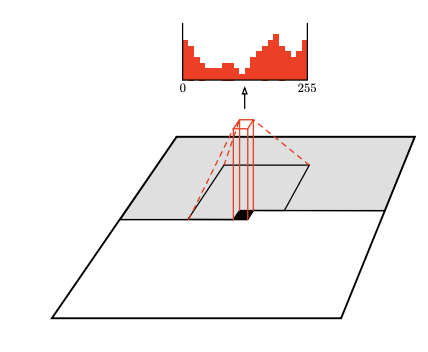
\includegraphics[scale=0.9]{images/masked_convolution_pixel_cnn}
    \caption{Masked convolution on an image (largest square), the big square represents the receptive field of the black pixel, the white area is masked}
    \label{fig:masked_convolution_pixel_cnn}
\end{figure}

Hence, given $x$ an image represented by its pixels $x = (x_1, \dots, x_n)$, as usual for these distribution modeling problems, we aim at finding $\theta^* = arg\max_{\theta} p_{\theta}(x)$ in a family of distributions parameterized by $\theta$: the maximum of likelihood.
Contrary to the usual independent framework, we consider a local dependency between pixels given by the receptive field of our convolution.
This local dependency is limited to the already seen pixels only as well, thanks to the masked convolution.
\medskip

Furthermore, rather than using continuous outputs, these architecture use a softmax layer to determine the pixel of a given generation,
leading to a discrete prior rather than a continuous one, which is required for the VQ-VAE for instance.
As a result, the distribution of a pixel conditionally to the ones in its receptive field is given by a multinomial in $\{0, \dots, 256\}$.
\medskip

\subsection{Usage in the VQ-VAE}

Once we have trained the VQ-VAE, the original paper states that we can replace the uniform prior on $p(z)$ by a PixelCNN to model the prior.
To perform the training of the PixelCNN, we turn the samples $x$ in their latent representations $z$, and train the PixelCNN over the latent representations $z$.
This way, we have created dependency between the $z$ in the latent feature mapping, and we obtain a prior over their distribution modeled by the PixelCNN.



% VQ Tree
\newpage
\section{Microbiota analysis}

This section aims at using the previous elements to design microbiota adapted latent methods.
\subsection{Microbiota dataset}

As we look into the microbiota data, we notice a major phylogenetic architecture to describe various levels of precision in the microbiota composition.
Indeed, such phylogenetic structure can be represented as a tree as on the following figure:
\begin{figure}[H]
    \center
    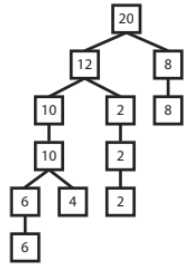
\includegraphics[scale=1]{images/abundance_tree_phylogenetic}
    \caption{Phylogenetic tree example with abundance data (in the nodes) at each layer of the tree.
    Each node represents a bacterium specie at a given precision layer in the tree. From \cite{microbiome_deeplearning_research}.}
    \label{fig:phylogenetic_tree}
\end{figure}

Such structure can not be used directly in a machine learning system since it's not a vectorizable representation.
Hence, we first suggest to transform the tree in a matrix to image structure as in the following example:
\begin{figure}[H]
    \center
    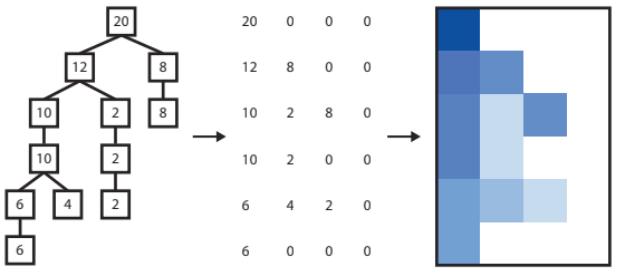
\includegraphics[scale=1]{images/tree_to_image}
    \caption{Phylogenetic tree to image representation:
    opacity of the pixel relates to the abundance of the species at the given level of precision (normalized between 0 and 1).
    From \cite{microbiome_deeplearning_research}.}
    \label{fig:phylogenetic_tree_to_img}
\end{figure}

Sadly this image representation does not convey the link between the species abundance given by the edges of the tree.
As a result, we suggest to find a hidden variable $Z$ that uses the adjacent matrix of the tree $T$, to find a way to go through the image
as for the PixelCNN approach.
Such approach, in addition to use the adjacency of the tree graph, would then learn an interesting trajectory to compute the correlation between the abundance data.
The next section offers the mathematical framework of the proposed idea.
\subsection{Simple generative model: no latent variable}

\subsubsection{Context and objective}

In first approximation, we would like to define a generative model that does not exploit any latent structure.
Such model, parameterized by $\theta$, aims at finding an optimal distribution in the sense of the maximum of likelihood,
within a family of distributions yet to be defined.
The maximum likelihood objective is given below as:
$$
\theta^* = arg\max_{\theta} p_{\theta}(X, T)
$$
One can rewrite the joint distribution as follow:
$$
\begin{align}
    p_{\theta}(X, T) &= \sum_{i=1}^n p_{\theta}(X_i, T_i) \\
                    &= \sum_{i=1}^n p_{\theta}(T_i) p_{\theta}(X_i | T_i)
\end{align}
$$

As a result, to compute this objective, we need to define a prior $p_{\theta}(T_i)$ that generates trees,
and a posterior distribution $p_{\theta}(X_i | T_i)$ that generates abundance data from a sampled tree.

\subsubsection{Design of the prior}

We aim at defining a parameterized distribution $p_{\theta}(T)$ from which one can sample trees.
We would also like this distribution to model the trees of the microbiota dataset, meaning that
the generated trees should look like the ones from the dataset as well, and respect the phylogenetic constraints. \\

Consequently, we introduce this first simple generative process to characterize $p_{\theta}(T)$:
\begin{algorithm}[H]
    \caption{Independent Branches Tree (IBT) sampling}
    \begin{algorithmic}
        \STATE Define the tree $T$
        \STATE Sample $K \sim \mathcal{B}(D, \pi)$ the number of leaf entities in the tree
        \For{$i \in \{1, \dots, K\}$}
            \STATE \quad Define the branch $b_i$
            \STATE \quad Set the root of the tree to the lowest precision level entity as $u_0^{(i)}$
            \STATE \quad Define $j = 0$
            \While{$u_{j}^{(i)}$ is not the empty node index}
                \STATE \quad \quad Append the node $u_{j}^{(i)}$ to the branch $b_i$
                \STATE \quad \quad Gather the possible children of the node $u_{j}^{(i)}$ as $V_{j}^{(i)}$
                \STATE \quad \quad Append the empty node index in $V_{j}^{(i)}$
                \STATE \quad \quad Sample $u_{j+1}^{(i)}$ following $g_{\pi_{u_{j}^{(i)}}}$ a discrete distribution over $V_{j}^{(i)}$ with weights $\pi_{u_{j}^{(i)}}$
                \STATE \quad \quad $j \leftarrow j + 1$
            \EndWhile
            \STATE \quad Add the branch $b_i$ to the tree $T$.
        \EndFor
        \RETURN{$T$}
    \end{algorithmic}
    \label{alg:algorithm}
\end{algorithm}

The IBT generates trees with independent branches, so that each node in a branch is dependent from the previous ones,
while each branch starts from the same root and are i.i.d.
Hence, such structure is one the most simple one could think of when generating trees. \\
Another step would be to add dependency between branches, for instance looking at each generation level what other entities
have been selected in all the branches at the same level before.
Though that would require a supplementary modelization step that we leave on the side for now. \\

Following the IBT modelization, we can compute the prior as:
$$
\begin{align}
    p_{\theta}(T) &= p_{\theta}(b_1, \dots, b_{|T|}) \\
                &= \prod_{i=1}^{|T|} p_{\theta}(b_i) \\
                &= \prod_{i=1}^{|T|} p_{\theta}(u_1^{(i)}, \dots, u_{|b_i|}^{(i)}) \\
                &= \prod_{i=1}^{|T|} \underbrace{p(u_1^{(i)})}_{1} p_{\pi_{u_1^{(i)}}}(u_2^{(i)} | u_1^{(i)}) \dots p_{\pi_{u_{|b_i|-1}^{(i)}}}(u_{|b_i|}^{(i)} | u_{|b_i|-1}^{(i)}) \\
                &= \prod_{i=1}^{|T|} \prod_{j=1}^{|b_i|-1} p_{\pi_{u_j^{(i)}}}(u_{j+1}^{(i)} | u_{j}^{(i)}) \\
                &= \prod_{i=1}^{|T|} \prod_{j=1}^{|b_i|-1} \pi_{u_j^{(i)} \rightarrow u_{j+1}^{(i)}} \right
\end{align}
$$

\subsubsection{Design of the posterior}

Now that we have a way to generate trees, we need to define an explicit stochastic relationship between the abundance
data and the structure of the tree.
Such inevitably exists, as when observing $T$, the abundance of an entity that isn't present in $T$ is necessarily 0.
Similarly, it is highly likely that when observing the presence of certain entities in $T$ that induces a high abundance of
another neighbour entity (interaction between bacteria). \\

Hence, since we would like an explicit model here, we will design a posterior $p_{\theta}(X|T)$ at each precision level
using a parametric distributions like the Dirichlet distribution. We assume the following framework:
\begin{itemize}
    \item We denote $X^{(l)} = (x_l^{(1)}, \dots, x_{l}^{(U_l)})$ the abundance vector at layer $l$.
    \item $X^{(1)} = (1)$ since it's the root of the tree.
    \item $X^{(2)} \sim \mathcal{D}(\alpha_2)$
    \item $\forall l \geq 3, X^{(l)} \sim \mathcal{D}(\alpha_l)$ if there's more than one node in the layer.
        Each value in $X^{(l)}$ is constrained by the following set of constraint $\mathcal{C}$:
        \begin{itemize}
              \item If node $k$ at layer $l-1$ has one child, then its abundance value is the same for the child node.
              \item If node $k$ at layer $l-1$ has at least two children, the children abundance sums to the parent's abundance value.
        \end{itemize}
        Hence, we obtain the following conditional distribution:
        $$
        \begin{align}
            p_{\gamma}(X^{(l+1)} | X^{(l)}) &= \frac{p_{\gamma}(X^{(l+1)}, X^{(l)})}{p_{\alpha_l}(X^{(l)})} \\
                                            &= \frac{p_{\alpha_{l+1}}(X^{(l+1)})}{p_{\alpha_{l}}(X^{(l)})} p(X^{(l)} | X^{(l+1)}) \\
                                            &= \frac{p_{\alpha_{l+1}}(X^{(l+1)})}{p_{\alpha_{l}}(X^{(l)})} \mathbbm{1}_{\mathcal{C}}
        \end{align}
        $$
\end{itemize}
% \subsection{Variational Tree Walk}

\subsubsection{EM approach}

In first approximation, we would like to use the EM algorithm to try to compute the following latent model:
\begin{itemize}
    \item We assume that we have $n$ individuals observed through $(X_i, T_i)_{1 \leq i \leq n}$.
    \item The maximum depth of a phylogenetic tree is $D$, the maximum number of nodes $N_T$, and the maximum amount of unique species at any level is $U$.
    \item $X_i$ is the abundance matrix of the individual $i$ (image of size $D \times U$) , which is observed.
    \item $T_i$ is the adjacent matrix of the phylogenetic tree of individual $i$, of size $N_T \times N_T$, which is observed.
          We could use any other encoding of a tree (contour function, depth function, ...).
    \item $Z_i$ is a hidden random walk over the tree $T_i$ (discrete vector, permutation of $(1, \dots, N_T)$).
          For a given random walk process over the tree, we denote by $N_{Z}$ the amount of possible generations ($N_Z \leq N_T!$).
          Hence, $p_{\gamma}(Z_i = z | T_i)$ is a known distribution defined by the random walk process.
    \item Taking inspiration from the PixelCNN, our model should learn the distribution $p_{\omega}(X_i | Z_i, T_i)$ as a CNN/RNN that is masked following $Z_i$.
          We also assume that conditionally to $Z_i$, this distribution is independent from the adjacent matrix: $p_{\omega}(X_i | Z_i, T_i) = p_{\omega}(X_i | Z_i)$.
\end{itemize}

Recall from the EM context that we aim at maximizing
$$
Q(\widehat{\theta}, \theta) = \mathbb{E}_{p_{\widehat{\theta}(Z|X,T)}}[\log p_{\theta}(X, Z, T) | X,T]
$$
Hence, we start with the \textbf{expectation} step and try to evaluate $p_{\widehat{\theta}}(Z|X,T)$:
$$
\begin{align}
    \log p_{\widehat{\theta}}(Z_i|X_i,T_i) = \tau_{ik} &= \log \frac{p(T_i) p_{\widehat{\theta}}(Z_i | T_i) p_{\widehat{\theta}}(X_i | Z_i, T_i)}{\sum_{j=1}^{N_Z} p(T_i) p_{\widehat{\theta}}(Z_i=z_j | T_i) p_{\widehat{\theta}}(X_i | Z_i=z_j, T_i)} \\
                                &= \log \frac{p_{\widehat{\theta}}(Z_i | T_i) p_{\widehat{\theta}}(X_i | Z_i)}{\sum_{j=1}^{N_Z} p_{\widehat{\theta}}(Z_i=z_j | T_i) p_{\widehat{\theta}}(X_i | Z_i=z_j)}
\end{align}
$$
Even though all terms seems computable and explicit here, the summation over $N_Z$ can be very large depending on the complexity of the random walk process we pick.
As a result, we will propose a variational approach to overcome this issue in the next section. \\

As it is right now, one could easily compute the \textbf{maximization} step for $Q(\widehat{\theta}, \theta)$ over $\theta = (\gamma, \omega)$, as it is now explicit:
$$
Q(\widehat{\theta}, \theta) = \sum_{i=1}^n (\log p(T_i) + \log p_{\gamma}(Z_i | T_i) + \log p_{\omega}(X_i | Z_i)) \tau_{ik}
$$

\subsubsection{Variational approach}

In this second approach, we aim at giving a variational algorithm to compute a lower bound to the true objective.
To that end, since it can not be computed directly, we propose an estimate of $p_{\theta}(Z|X,T) = q_{\Phi}(Z|X,T)$.
Recall then the ELBO explicited in the VAE general framework:
$$
\log p_{\theta}(X) = \underbrace{\mathbb{E}_{q_{\Phi}(Z|X,T)}\left[ \log \frac{p_{\theta}(X,Z,T)}{q_{\Phi}(Z|X,T)} \right]}_{ELBO(\Phi, \theta)} + D_{KL}[q_{\Phi}(Z|X,T) \Vert p_{\theta}(Z|X,T)]
$$
Such ELBO can be rewritten as:
$$
\begin{align}
    ELBO(\Phi, \theta) &= \mathbb{E}_{q_{\Phi}(Z|X,T)}[\log p_{\theta}(X,Z,T)] - \mathbb{E}_{q_{\Phi}(Z|X,T)}[\log q_{\Phi}(Z|X,T)] \\
                        &= \mathbb{E}_{q_{\Phi}(Z|X,T)}[\log p_{\theta}(X|Z,T)] - \mathbb{E}_{q_{\Phi}(Z|X,T)}\left[ \log \frac{q_{\Phi}(Z|X,T)}{p_{\gamma}(Z,T)} \right] \\
                        &= \mathbb{E}_{q_{\Phi}(Z|X,T)}[\log p_{\theta}(X|Z)] - D_{KL}[q_{\Phi}(Z|X,T) \Vert p_{\gamma}(Z|T)] + \log p(T)
\end{align}
$$

Designing the prior $p_{\gamma}(Z_i | T_i)$ is no easy task though, as it is completely free-form.
Indeed, using a too free-form prior will end up in not using the tree structure at all by creating a completely unrelated chain
(if any leap can be made in the tree, then the obtained random walk will not necessarily exploit the tree structure).
If the the prior is too restrictive, we might be over-exploiting the phylogenetic structure and obtain an average walk over the tree that is not relevant to each unique case.
Hence, we try to design a prior that takes into account the tree structure while still having some entropy so any random walk is still possible (with low probability).\\

For notation purposes, we introduce the random variable $z_k$ that represents the chosen node index at step $k$ of the random walk.
Whatever prior we decide to pick, it feels as most relevant to pick the seed of the chain using a learnable distribution,
so that we have $z_{1} \sim p(\pi_1)$ where $\pi_1 = (\pi_1^{(1)}, \dots, \pi_1^{(N_T)})$ .
We also introduce a norm over the tree $\Vert . \Vert_T$ that will enable us to measure the distance between nodes:
\begin{itemize}
    \item Norm of a given node is given by:
        $$
        \Vert z_k \Vert_T = \text{distance to root node of the tree}
        $$
    \item Distance computation is given by:
          $$
            \Vert z_k - z_j \Vert_T = \left\{
            \begin{array}{ll}
                0 & \mbox{if } i = j \\
                1 & \mbox{if } i \neq j \mbox{ and nodes have the same parent} \\
                \text{number of edges between node $k$ and $j$} & \mbox{otherwise}
            \end{array}
            \right.
          $$
\end{itemize}

The first prior that we propose is a variation of the dirichlet prior, parameterized by $\lambda = (\lambda_1, \dots, \lambda_{N_T})$.
If we denote by $u_k$ a given node indexed by $k$, let $\alpha_j = (\Vert u_k - z_j \Vert_T)_{1 \leq k \leq N_T}$:
$$
\begin{align}
    \pi_{k+1} | z_{k} &\sim \mathcal{D}(\lambda \odot \alpha_k) \\
    z_{k+1} | \pi_{k+1} &\sim p(\pi_{k+1})
\end{align}
$$
Hence, computing $Z_i | T_i$ is given by $Z_i = (z_k)_{k \in \{1, \dots, N_T\}}$ following the previously introduced process:
\begin{algorithm}[H]
    \caption{Tree random walk without replacement}
    \begin{algorithmic}[1]
        \REQUIRE $T_i$ a given tree, $(\pi_1, \lambda)$ distribution parameters
        \STATE Draw $z_{1} \sim p(\pi_1)$
        \STATE Define $Z_i = (z_{1})$
        \For{ $k \in \{2, \dots, N_T\}$ }
            \STATE \quad Draw a distribution $\pi_{k} | z_{k-1} \sim \mathcal{D}(\lambda \odot \alpha_{k-1})$
            \STATE \quad Mask in $\pi_{k}$ the already seen nodes in $Z_i$ to obtain $\tilde{\pi}_{k}$
            \STATE \quad Draw $z_{k} \sim p(\tilde{\pi}_{k})$
            \STATE \quad Update $Z_i = (Z_i, z_k)$
        \EndFor:

        \RETURN{} $Z_i = (z_1, \dots, z_{N_T})$, $\pi = (\pi_1, \dots, \pi_k)$
    \end{algorithmic}


    \label{alg:tree_walk_no_replacement}
\end{algorithm}

Computing $q_{\Phi}(Z_i | X_i, T_i)$ is not so simple at this stage, and it does not have an explicit formula:
$$
\begin{align}
    q_{\Phi}(Z_i = (z_1, \dots, z_{N_T}), \Pi | X_i, T_i) &= p_{\Phi}(z_1, \dots, z_{N_T}, \pi_1, \dots, \pi_{N_T}) \\
                                                                &= p_{\Phi}(z_1, \pi_1) p_{\Phi}(z_2, \pi_2 | z_1, \pi_1) \dots p_{\Phi}(z_{N_T}, \pi_{N_T} | z_{1:N_T-1}, \pi_{1:N_T-1}) \\
                                                                &= p(\pi_1) p(z_1 | \pi_1) \prod_{k=2}^{N_T} p(\pi_{k} | z_{1:k-1}, \pi_{1:k-1}) p(z_{k} | \pi_{1:k}, z_{1:k-1}) \\
                                                                &= p(z_1 | \pi_1) \prod_{k=2}^{N_T} p(\pi_k | z_{k - 1}) p(z_{k} | \pi_{k}, z_{1:k}) \\
                                                                &= p(z_1 | \pi_1) \prod_{k=2}^{N_T} p_{\lambda}(\pi_k ; \alpha_{k - 1}) p(z_{k} | \tilde{\pi}_{k}) \\
\end{align}
$$
Leading to:
$$
\begin{align}
    q_{\Phi}( z | X_i, T_i) &= \int_{\mathbold{\Pi}}  q_{\Phi}((z_1, \dots, z_{N_T}), \pi | X_i, T_i) d\pi \\
                            &= \int_{\mathbold{\Pi}}  p(z_1 | \pi_1) \prod_{k=2}^{N_T} p_{\lambda}(\pi_k ; \alpha_{k - 1}) p(z_{k} | \tilde{\pi}_{k}) d\pi_1 \dots d\pi_{N_T} \\
                            &= \int_{\mathbold{\Pi}_1} \pi_1^{(z_1)} \int_{\mathbold{\Pi}_2} p_{\lambda}(\pi_2;\alpha_1) \mathbbm{1}_{z_2 \notin \{z_1\}} \pi_{2}^{(z_2)} \dots \int_{\mathbold{\Pi}_{N_T}} p_{\lambda}(\pi_{N_T};\alpha_{N_T - 1}) \mathbbm{1}_{z_{N_T} \notin \{z_1, \dots, z_{N_T-1}\}} \pi_{N_T}^{(z_{N_T})} d\pi_{1:N_T} \\
                            &= \prod_{k=2}^{N_T} \mathbbm{1}_{z_{k} \notin \{z_{1}, \dots, z_{k-1}\}} \int_{\mathbold{\Pi}_2} p_{\lambda}(\pi_2;\alpha_1) \pi_{2}^{(z_2)} \dots \int_{\mathbold{\Pi}_{N_T}} p_{\lambda}(\pi_{N_T};\alpha_{N_T - 1}) \pi_{N_T}^{(z_{N_T})} d\pi_{1:N_T} \\
\end{align}
$$
Since we are using the dirichlet distribution, its components are independent so that $p_{\lambda}(\pi_k;\alpha_{k-1}) = \frac{1}{B(\alpha_{k-1})} \prod_{i=1}^{N_T} \left(\pi_k^{(i)}\right)^{\alpha_{k-1}^{(i)} - 1}$.
Hence, using Fubini-Tonelli theorem and the first order moment of the dirichlet distribution, we get for all $k \geq 2$:
$$
\begin{align}
    \int_{\mathbold{\Pi}_k} p_{\lambda}(\pi_k;\alpha_{k-1}) \pi_{k}^{(z_k)} d\pi_{k} &= \int_{\mathbold{\Pi}_k} \frac{1}{B(\alpha_{k-1})} \prod_{i=1}^{N_T} \left(\pi_k^{(i)}\right)^{\alpha_{k-1}^{(i)} - 1} \pi_{k}^{(z_k)} d\pi_{k}^{(1:N_T)} \\
                                                                                     &= \frac{1}{B(\alpha_{k-1})} \int_{\mathbold{\Pi}_k^{(z_k)}} \left(\pi_k^{(z_k)}\right)^{\alpha_{k-1}^{(z_k)}-1} \pi_k^{(z_k)} d\pi_k^{(z_k)} \prod_{i=0, i \neq z_k}^{N_T} \int_{\mathbold{\Pi}_k^{(i)}} \left(\pi_k^{(i)}\right)^{\alpha_{k-1}^{(i)}-1} d\pi_{k}^{(i)} \\
                                                                                     &= \frac{1}{B(\alpha_{k-1})} \int_{\mathbold{\Pi}_k^{(z_k)}} \left(\pi_k^{(z_k)}\right)^{\alpha_{k-1}^{(z_k)}} d\pi_k^{(z_k)} \prod_{i=0, i \neq z_k}^{N_T} \frac{1}{\alpha_{k-1}^{(i)}} \\
                                                                                     &= \frac{1}{B(\alpha_{k-1})} \frac{1}{\alpha_{k-1}^{(z_k)} + 1} \prod_{i=0, i \neq z_k}^{N_T} \frac{1}{\alpha_{k-1}^{(i)}}
\end{align}
$$
Consequently, $q_{\Phi}( z | X_i, T_i)$ can be written as:
$$
q_{\Phi}(Z_i = (z_1, \dots, z_{N_T}) | X_i, T_i) = \prod_{k=2}^{N_T} \mathbbm{1}_{z_{k} \notin \{z_{1}, \dots, z_{k-1}\}} \prod_{k=2}^{N_T} \left[  \frac{1}{B(\alpha_{k-1})} \frac{1}{\alpha_{k-1}^{(z_k)} + 1} \prod_{i=0, i \neq z_k}^{N_T} \frac{1}{\alpha_{k-1}^{(i)}} \right]
$$

Taking inspiration from the VQ-VAE architecture, one might modify the previous algorithm as simple prior sampling denoted by $Z_i^e(T_i)$,
and then a quantization step by taking the $arg\max$ over the output probabilities sampled:
$$
\begin{align}
    \pi_{k+1} | z_{k} &\sim \mathcal{D}(\lambda \odot \alpha_k) \\
    z_{k+1} &= arg\max_{j} \pi_{k+1}^{(j)}
\end{align}
$$

\begin{algorithm}[H]
    \caption{Tree quantized random walk}
    \begin{algorithmic}
        \REQUIRE $T_i$ a given tree, $(\pi_1, \lambda)$ distribution parameters
        \STATE Draw $z_{1} \sim p(\pi_1)$
        \STATE Define $Z_i^q = (z_{1})$
        \For{ $k \in \{2, \dots, N_T\}$ }
            \STATE \quad Draw a distribution $\pi_{k} | z_{k-1} \sim \mathcal{D}(\lambda \odot \alpha_{k-1})$
            \STATE \quad Mask in $\pi_{k}$ the already seen nodes in $Z_i^q$ to obtain $\tilde{\pi}_{k}$
            \STATE \quad Set $z_{k} = arg\max_{j} \tilde{\pi}_{k}^{(j)}$
            \STATE \quad Update $Z_i^q = (Z_i^q, z_k)$
        \EndFor:

        \RETURN{} $Z_i^q = (z_1, \dots, z_{N_T})$
    \end{algorithmic}

    \label{alg:tree_quantized_walk}
\end{algorithm}

Sadly, $q_{\Phi}(Z_i|X_i,T_i) \neq \delta_{\{Z_i = Z_i^q\}}$, so we do not fall back on that objective yet:
$$
\begin{align}
    ELBO(\Phi, \theta) &= \sum_{i=1}^n \log p_{\omega}(X_i | Z_i^q(T_i)) - \log \frac{q_{\Phi}(Z_i^q(T_i) | X_i)}{p_{\gamma}(Z_i^q (T_i) | T_i)} \\
    &= \sum_{i=1}^n \log p_{\omega}(X_i | Z_i^q(T_i)) + \log p_{\gamma}(Z_i^q (T_i) | T_i)
\end{align}
$$

Being a random process, the density of a moving random process is yet to be defined.

\newpage
\section{Bibliography}
% \pagebreak
\nocite{*}
\printbibliography

\end{document}